\documentclass[12pt]{article}
%pdflatex -shell-escape informe.tex 


% --- Paquetes básicos ---
\usepackage[utf8]{inputenc}
\usepackage[T1]{fontenc}
\usepackage[spanish, provide=*]{babel}
\usepackage{geometry}
\usepackage{hyperref}
\usepackage{subcaption}  % En el preámbulo
\geometry{a4paper, margin=2.5cm}
\setlength{\headheight}{14.5pt}
\addtolength{\topmargin}{-2.5pt}

% --- Carátula ---
\title{Python Inicial}
\author{Jose Miguel Paz Portilla\\Proyecto Final\\Inventario de Productos}
\date{\today}

% --- Código Python con minted ---
\usepackage{minted} % Requiere -shell-escape
\usemintedstyle{friendly}

% --- Otros paquetes útiles ---
\usepackage{graphicx}
\usepackage{fancyhdr}
\pagestyle{fancy}
\fancyhead[L]{Python Inicial}
\fancyhead[R]{\thepage}

\begin{document}

% Carátula
\maketitle
\thispagestyle{empty}
\newpage

% Índice
\tableofcontents
\newpage
%%%%%%%%%%%%%%%%%%%%%%%%%%%%%%%%%%%%%%%%%%%%%%%%%%%%%%%%%%%%%%%%%%%%%%%%%%%%%%%%%%%%%%%%%%%%%%%%%%%%%%%%%%%%%%%%%%%%%%%%%%%%%%%%%
\section{Introducción}

Con el objetivo de realizar un inventario de productos con persistencia de información, se desarrollo 2 versiones del programa escritos en python, uno con persistencia en archivo CSV y otro manejando una base de datos con SQL. \\

Los requisitos de CSV son:

\begin{enumerate}
	\item Usar listas para almacenar y gestionar los datos.
	\item Incorporar bucles while y for según corresponda. 
	\item Validar entradas del usuario o usuaria, asegurándote de que no se ingresen datos vacíos o incorrectos.
	\item Utilizar condicionales para gestionar las opciones del menú y las validaciones necesarias.
	\item Presentar un menú que permita elegir entre las funcionalidades disponibles: agregar productos, visualizar productos, buscar productos y eliminar productos.
	\item El programa debe continuar funcionando hasta que se elija una opción para salir.
	\item El programa persiste la información en un archivo del disco rígido el tipo CSV.
\end{enumerate}



%%%%%%%%%%%%%%%%%%%%%%%%%%%%%%%%%%%%%%%%%%%%%%%%%%%%%%%%%%%%%%%%%%%%%%%%%%%%%%%%%%%%%%%%%%%%%%%%%%%%%%%%%%%%%%%%%%%%%%%%%%%%%%%%%
\section{Implementación}

\subsection{Implementación CSV}

Utilizo la función main como función principal del programa, el cual muestra un menu con opciones al usuario, y según la opcion elegida realiza alguno de los requisitos solicitados.

Para ejecutar el programa desde una terminal ubicada donde se encuentran los \textbf{archivos python} y el \textbf{archivo makefile} ingresar \textit{make} o \textit{make run}, como muesta la \autoref{fig:Correr el programa}

\begin{figure}[H]
	\centering
	\setlength{\fboxrule}{0pt}
	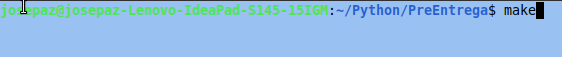
\includegraphics[width=0.66\textwidth]{Imagenes/img0.png}
	\caption{Como correr el programa desde terminal}
	\label{fig:Correr el programa}
\end{figure}  

Al iniciar el programa, si no hay un archivo CSV se inicializa la lista de productos como vacia, caso contrario se carga la lista de productos con los productos del archivo CSV.\\

El programa refresca la terminal y muestra un menu con opciones, se le solicita al usuario que ingrese un número del menu entre las disponibles, como se muestra en la \autoref{fig:menu}.

\begin{figure}[H]
	\centering
	\setlength{\fboxrule}{0pt}
	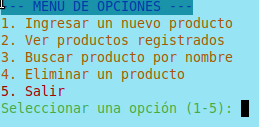
\includegraphics[width=0.35\textwidth]{Imagenes/menu.png}
	\caption{Mostrando el menu}
	\label{fig:menu}
\end{figure} 

Al ingresar la opción $1$, se solicita el nombre, categoria y precio del \textbf{nuevo producto} para almacenarlo en la lista productos, como se muentra en la \autoref{fig:nuevo producto}.

\begin{figure}[H]
	\centering
	\setlength{\fboxrule}{0pt}
	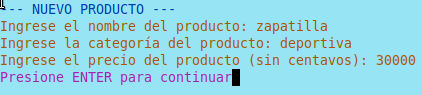
\includegraphics[width=0.5\textwidth]{Imagenes/nuevo_producto.png}
	\caption{Ingreso nuevo producto}
	\label{fig:nuevo producto}
\end{figure} 

Posteriormente al ingresar la opción $2$, a partir de la lista productos se muestran los productos del inventario, como se observa en la \autoref{fig:mostrar productos}.

\begin{figure}[H]
	\centering
	\setlength{\fboxrule}{0pt}
	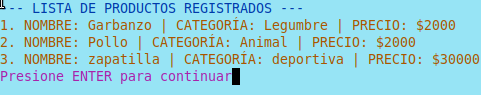
\includegraphics[width=0.5\textwidth]{Imagenes/mostrar_productos.png}
	\caption{Mostrar productos}
	\label{fig:mostrar productos}
\end{figure} 

Para buscar un producto por su nombre se ingresa la opcion $3$, el programa busca en la lista del inventario y va almacenando en una lista auxiliar todos los productos que coinciden con el nombre del producto, y lo muestra por la terminal, como se muestra en la \autoref{fig:buscar producto}.

\begin{figure}[H]
	\centering
	\setlength{\fboxrule}{0pt}
	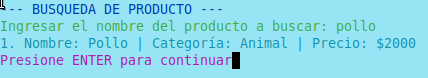
\includegraphics[width=0.5\textwidth]{Imagenes/busqueda_por_nombre_producto.png}
	\caption{Buscar producto por nombre}
	\label{fig:buscar producto}
\end{figure} 

Con la opción $4$, se puede eliminar un producto con la posición en la lista mostrada por terminal, como se muestra en \autoref{fig:eliminar producto}.

\begin{figure}[H]
	\centering
	\setlength{\fboxrule}{0pt}
	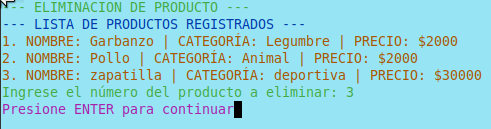
\includegraphics[width=0.5\textwidth]{Imagenes/eliminar_producto.png}
	\caption{Eliminar producto por indice}
	\label{fig:eliminar producto}
\end{figure} 

Finalmente para finalizar el programa se ingresa la opción $5$, y se muestra por terminal un mensaje de finalización, como en la \autoref{fig:fin programa}.
\begin{figure}[H]
	\centering
	\setlength{\fboxrule}{0pt}
	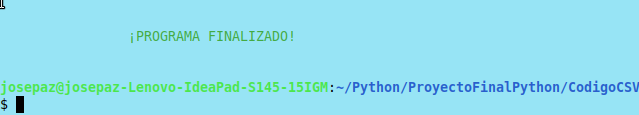
\includegraphics[width=0.66\textwidth]{Imagenes/finalizar_programa.png}
	\caption{Finalizacion del programa}
	\label{fig:fin programa}
\end{figure} 

Además se muestra el archivo CSV que actua como base de datos, como se observa en la \autoref{fig:archivo_csv}.

\begin{figure}[H]
	\centering
	\setlength{\fboxrule}{0pt}
	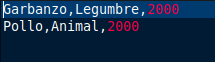
\includegraphics[width=0.3\textwidth]{Imagenes/archivo_csv.png}
	\caption{Archivo CSV}
	\label{fig:archivo_csv}
\end{figure} 


\subsection{Implementación SQL}
Aún no se vio el tema.
%%%%%%%%%%%%%%%%%%%%%%%%%%%%%%%%%%%%%%%%%%%%%%%%%%%%%%%%%%%%%%%%%%%%%%%%%%%%%%%%%%%%%%%%%%%%%%%%%%%%%%%%%%%%%%%%%%%%%%%%%%%%%%%%%
\section{Pruebas}

\subsection{Pruebas CSV}
\subsubsection{Opción fuera del rango}

Como se observa en la \autoref{fig:error rango de opciones}, al ingresar una opción fuera de las opciones del menu 
el programa evita que se ejecuten.

\begin{figure}[H]
	\centering
	\setlength{\fboxrule}{0pt}
	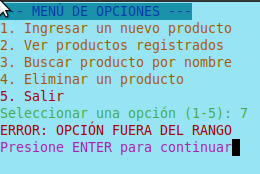
\includegraphics[width=0.3\textwidth]{Imagenes/error_opcion_menu.png}
	\caption{Error por elegir opciones fuera del rango}
	\label{fig:error rango de opciones}
\end{figure} 

\subsubsection{Campos del producto}

Como se observa en la \autoref{fig:error en campos de producto}, al ingresar campos vacios del nombre o categoria del producto o bien si se 
ingresa valores no enteros al precio del producto, el sistema no permite continuar con la ejecución del programa.

\begin{figure}[H]
	\centering
	\setlength{\fboxrule}{0pt}
	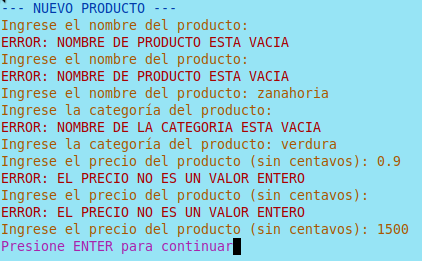
\includegraphics[width=0.6\textwidth]{Imagenes/errores_nuevo_producto.png}
	\caption{Pruebas al ingresar los campos del producto}
	\label{fig:error en campos de producto}
\end{figure} 

\subsubsection{Busqueda de producto por nombre}

Al ingresar varios productos, se guardan en la lista de productos en forma ordenada alfabeticamente por nombre. Cuando se busca un nombre de un producto
se genera una sublista con las coincidencias y se muestra por la terminal en caso en encontrar como se muestra en la \autoref{fig:busqueda de producto}, sino muestra un mensaje que el producto no esta en el inventario.

\begin{figure}[H]
    \centering

    \begin{subfigure}[b]{0.6\textwidth}
        \centering
        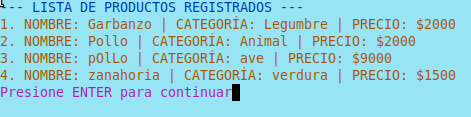
\includegraphics[width=\textwidth]{Imagenes/productos_pre_busqueda.png}
        \caption*{(a) Productos en el inventario}
    \end{subfigure}
    \hfill
    \begin{subfigure}[b]{0.6\textwidth}
        \centering
        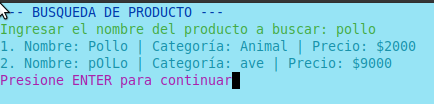
\includegraphics[width=\textwidth]{Imagenes/productos_post_busqueda.png}
        \caption*{(b) Busqueda de un producto por nombre encontrado}
    \end{subfigure}

    \caption{Busqueda de producto por  nombre}
    \label{fig:busqueda de producto}
\end{figure}

\subsubsection{Eliminación de producto por posición}

Como se muestra en la \autoref{fig:eliminacion de producto}, en la terminal se observan los productos que hay en el inventario, junto a un numero, para eliminar por ejemplo naranja, se ingresa su posición en la lista mostrada que es $3$, luego se vuelve a mostrar los productos y se observa que fue eliminado del inventario.
\begin{figure}[H]
    \centering

    \begin{subfigure}[b]{0.6\textwidth}
        \centering
        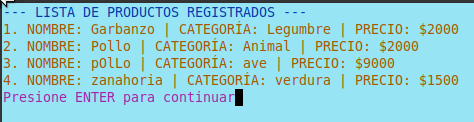
\includegraphics[width=\textwidth]{Imagenes/pre_eliminacion.png}
        \caption*{(a) Posición del producto a eliminar}
    \end{subfigure}
    \hfill
    \begin{subfigure}[b]{0.6\textwidth}
        \centering
        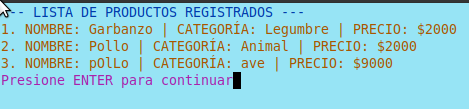
\includegraphics[width=\textwidth]{Imagenes/post_eliminacion.png}
        \caption*{(b) Inventario despues de eliminar el producto}
    \end{subfigure}

    \caption{Eliminación de producto por posición en el menú}
    \label{fig:eliminacion de producto}
\end{figure}


%%%%%%%%%%%%%%%%%%%%%%%%%%%%%%%%%%%%%%%%%%%%%%%%%%%%%%%%%%%%%%%%%%%%%%%%%%%%%%%%%%%%%%%%%%%%%%%%%%%%%%%%%%%%%%%%%%%%%%%%%%%%%%%%%
\section{Código}
\subsection{Código - CSV = Comma Separated Values(Valores Separados por Coma)}

\subsubsection{makefile}
\inputminted[fontsize=\small]{make}{CodigoCSV/makefile}

\subsubsection{main.py}
\inputminted[fontsize=\small, breaklines=true]{python}{CodigoCSV/main.py}

\subsubsection{menu.py}
\inputminted[fontsize=\small, breaklines=true]{python}{CodigoCSV/menu.py}

\subsubsection{opciones.py}
\inputminted[fontsize=\small, breaklines=true]{python}{CodigoCSV/opciones.py}

\subsubsection{metodos\_productos.py}
\inputminted[fontsize=\small, breaklines=true]{python}{CodigoCSV/metodos_productos.py}
%%%%%%%%%%%%%%%%%%%%%%%%%%%%%%%%%%%%%%%%%%%%%%%%%%%%%%%%%%%%%%%%%%%%%%%%%%%%%%%%%%%%%%%%%%%%%%%%%%%%%%%%%%%%%%%%%%%%%%%%%%%%%%%%%
\subsection{Código - SQL = Structured Query Language(Lenguaje de Consulta Estructurado)}

\subsubsection{makefile}
\inputminted[fontsize=\small]{make}{CodigoSQL/makefile}

\subsubsection{main.py}
\inputminted[fontsize=\small, breaklines=true]{python}{CodigoSQL/main.py}

\subsubsection{menu.py}
\inputminted[fontsize=\small, breaklines=true]{python}{CodigoSQL/menu.py}

\subsubsection{productos.py}
\inputminted[fontsize=\small, breaklines=true]{python}{CodigoSQL/productos.py}
%%%%%%%%%%%%%%%%%%%%%%%%%%%%%%%%%%%%%%%%%%%%%%%%%%%%%%%%%%%%%%%%%%%%%%%%%%%%%%%%%%%%%%%%%%%%%%%%%%%%%%%%%%%%%%%%%%%%%%%%%%%%%%%%%
\section{Conclusión}

En este informe realizado al combinar \LaTeX y Python se presenta una simplificación del programa inventario, donde se pudo aplicar lo aprendido en clases, como listas, archivos,  condicionales, bucles, ademas se uso modulacion y funciones, además de el uso de la función main y un makefile para ejecutar de un forma más práctica el código.

\end{document}
